\section{Test des Reglers}

\subsection{Messdaten}

\begin{figure}[h!]
	\centering
	\begin{subfigure}{0.475\textwidth}
		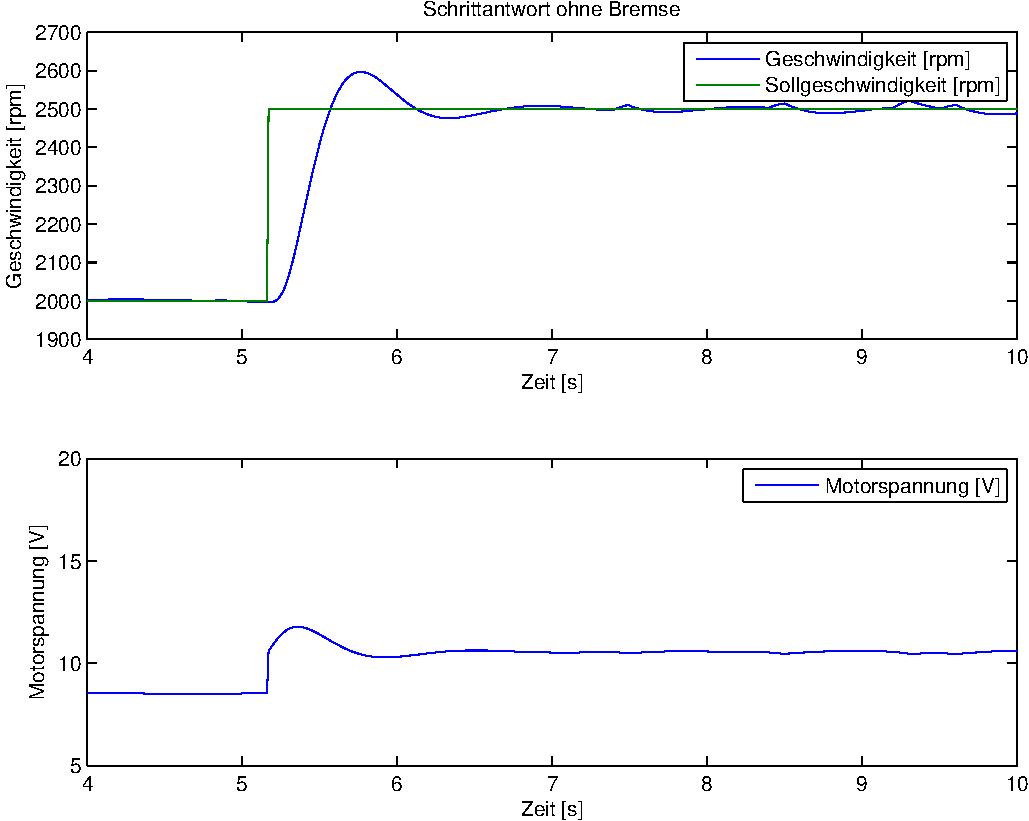
\includegraphics[width=1\textwidth]{12/step_noload.pdf}
		\caption{Ohne Bremse ($\alpha = 0$)}
	\end{subfigure}
	\hfill{}
	\begin{subfigure}{0.475\textwidth}
		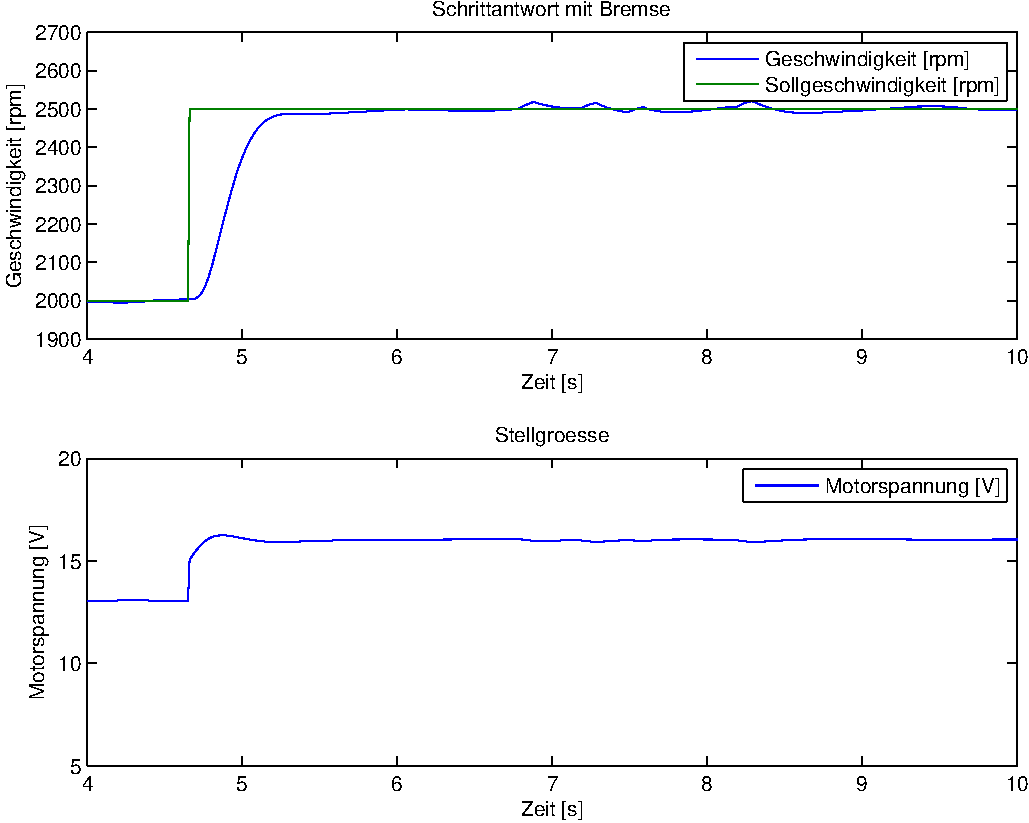
\includegraphics[width=1\textwidth]{12/step_load.pdf}
		\caption{Ohne Bremse ($\alpha = 0$)}
	\end{subfigure}
	\caption{Sprungantworten mit dem optimierten Regler}
\end{figure}


\begin{table}[h!]
	\centering
	\begin{tabular}{l c c c c}
		Eigenschaft
			& Spezifikation
			& $\alpha = 0$
			& $\alpha = 0.5$
			& Einheit \\
		\hline
		Genauigkeit (mean)
			& 100
			& 100 
			& 100
			& \% \\
		Anregelzeit (0-99\%)
			& $0.8$
			& 0.4
			& 1.2
			& $\si{\second}$ \\
		Überschwingen
			& $15$
			& 19.28
			& 0
			& \% \\
		Einschwingzeit
			& $2$
			& n.a. 
			& n.a.
			& $\si{\second}$ \\
	\end{tabular}
\end{table}
